\chapter{Week 3 -- MATLAB}

This report presents the results of tasks required by the assignment\footnote{accesiable via \vomihwassignment}. The exercise focused on the basics of the MATLAB environment and its utilization for processing of large datasets. As an illustration, the report demonstrated results from processing a dataset of several cell charge/discharge cycles.

\section{Abstract}

\section{Experimental results}

Table \ref{tab:3-dchg-cap} lists discharge capacities recorded during individual cycles.

\begin{table}[htbp]
    \centering
    \begin{tabular}{|c|c|c|c|c|c|c|}
    \hline
         cycle ID & 1 & 2 & 3 & 4 & 5 & 6 \\\hline
         Discharging capacity Q [Ah] &  3.163   &    3.1505       & 3.1311  &     3.1164   &    3.1049      & 3.2172 \\\hline
    \end{tabular}
    \caption{Discharging capacity available at each recorded cycle}
    \label{tab:3-dchg-cap}
\end{table}

\begin{figure}[htbp]
    \centering
    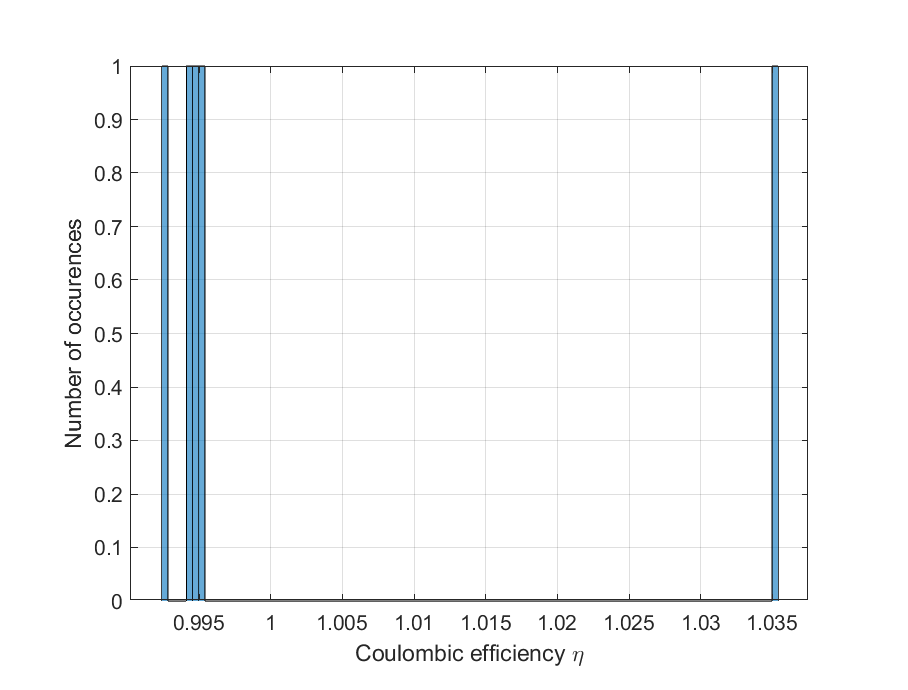
\includegraphics[width=0.75\linewidth]{figures/3/etas.eps}
    \caption{Histogram of coulombic efficiencies $\eta$ from completed cycles}
    \label{fig:3-etas}
\end{figure}

Histogram of coulombic efficiencies recorded for individual cycles is show in Fig. \ref{fig:3-etas}. It only shows data from complete cycles (i.e. without the first cycle). An interesting detail is the occurrence of number greater than one -- this $\eta$ corresponds to the last cycle, where a significantly lower current of 1 A (compared to previously used 3 A) was used to discharge the cell. Lower current lead to lower terminal voltage drop when loaded and therefore the cell was able to discharge more charge before the cycle ended safely. Otherwise the efficiency can't be higher than 1. The state of charge at each time during the experiment is shown in Fig. \ref{fig:3-soc}.


\begin{figure}[htbp]
    \centering
    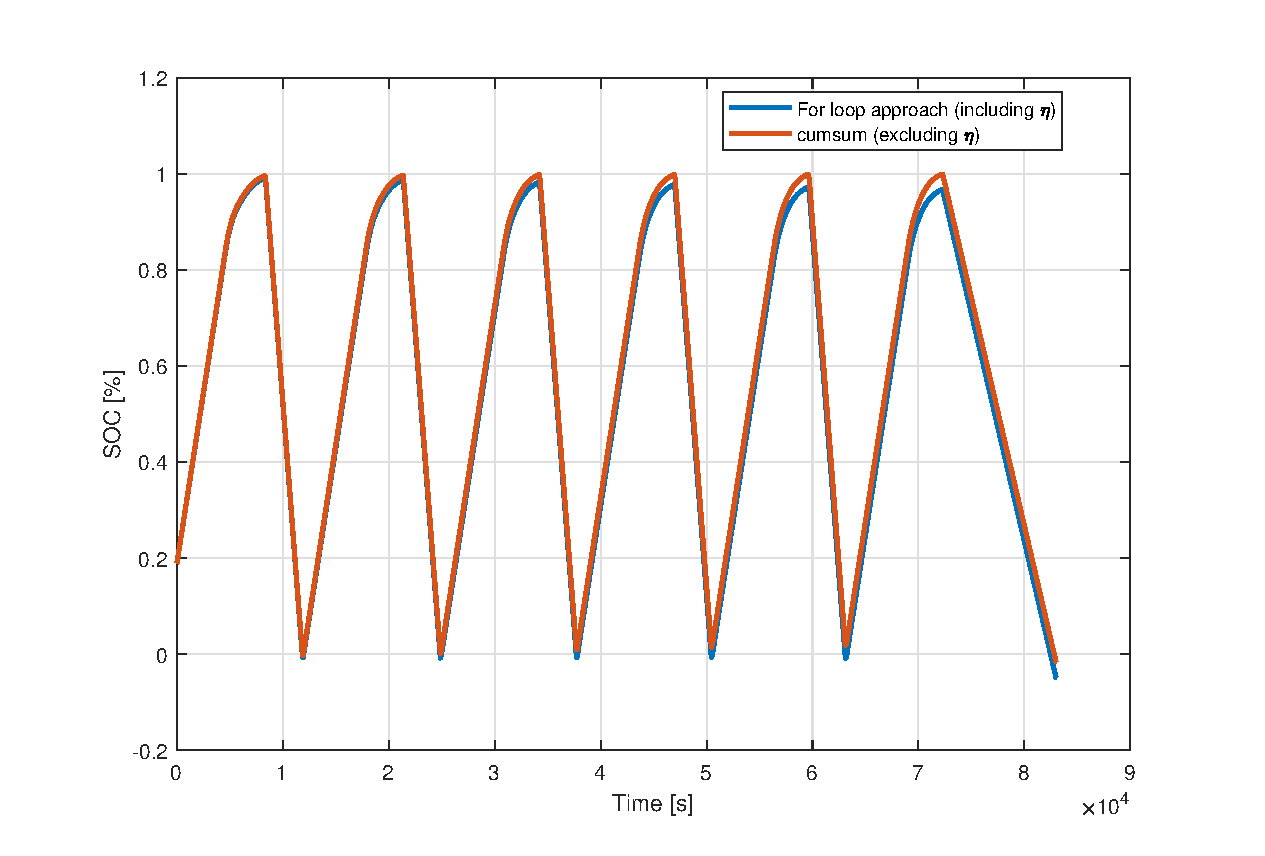
\includegraphics[width=0.75\linewidth]{figures/3/soc.eps}
    \caption{State of charge calculated using two different methods}
    \label{fig:3-soc}
\end{figure}

Cell data from the second charge-discharge cycle are shown in Fig. \ref{fig:3-tiled-layout}, clearly showing the CC-CV charging mode and the successive CC discharge.

\begin{figure}[htbp]
    \centering
    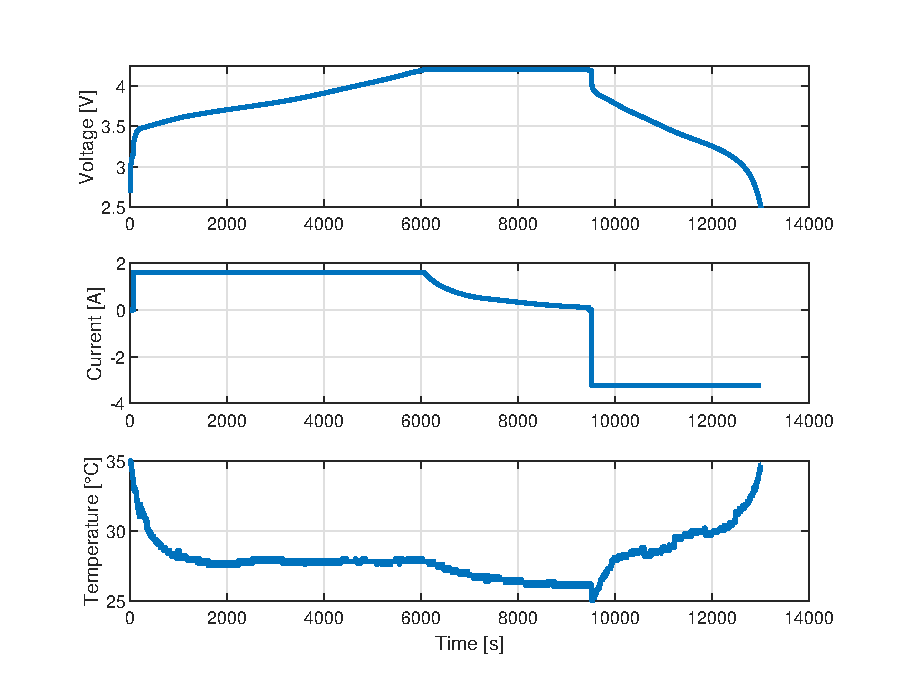
\includegraphics[width=0.75\linewidth]{figures/3/tiledlayout.eps}
    \caption{Voltage, current and temperature of cell during second charge-discharge cycle}
    \label{fig:3-tiled-layout}
\end{figure}



\begin{figure}[htbp]
    \centering
    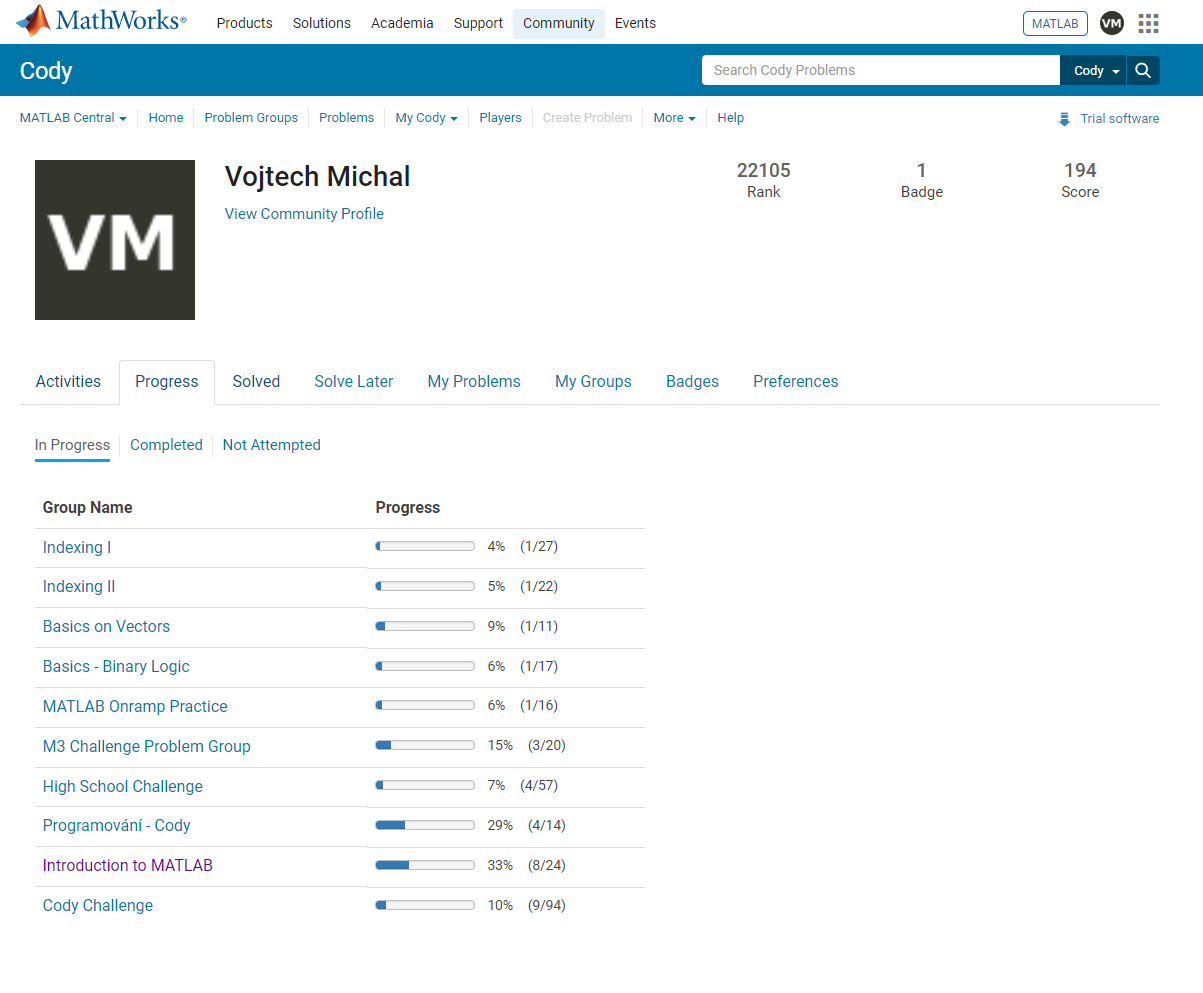
\includegraphics[width=0.99\linewidth]{figures/3/Cody.png}
    \caption{Proof of finished Matlab Cody exercises}
    \label{fig:3-cody}
\end{figure}
